\documentclass{standalone}
\usepackage{tikz}
\usetikzlibrary{patterns, positioning}


\begin{document}
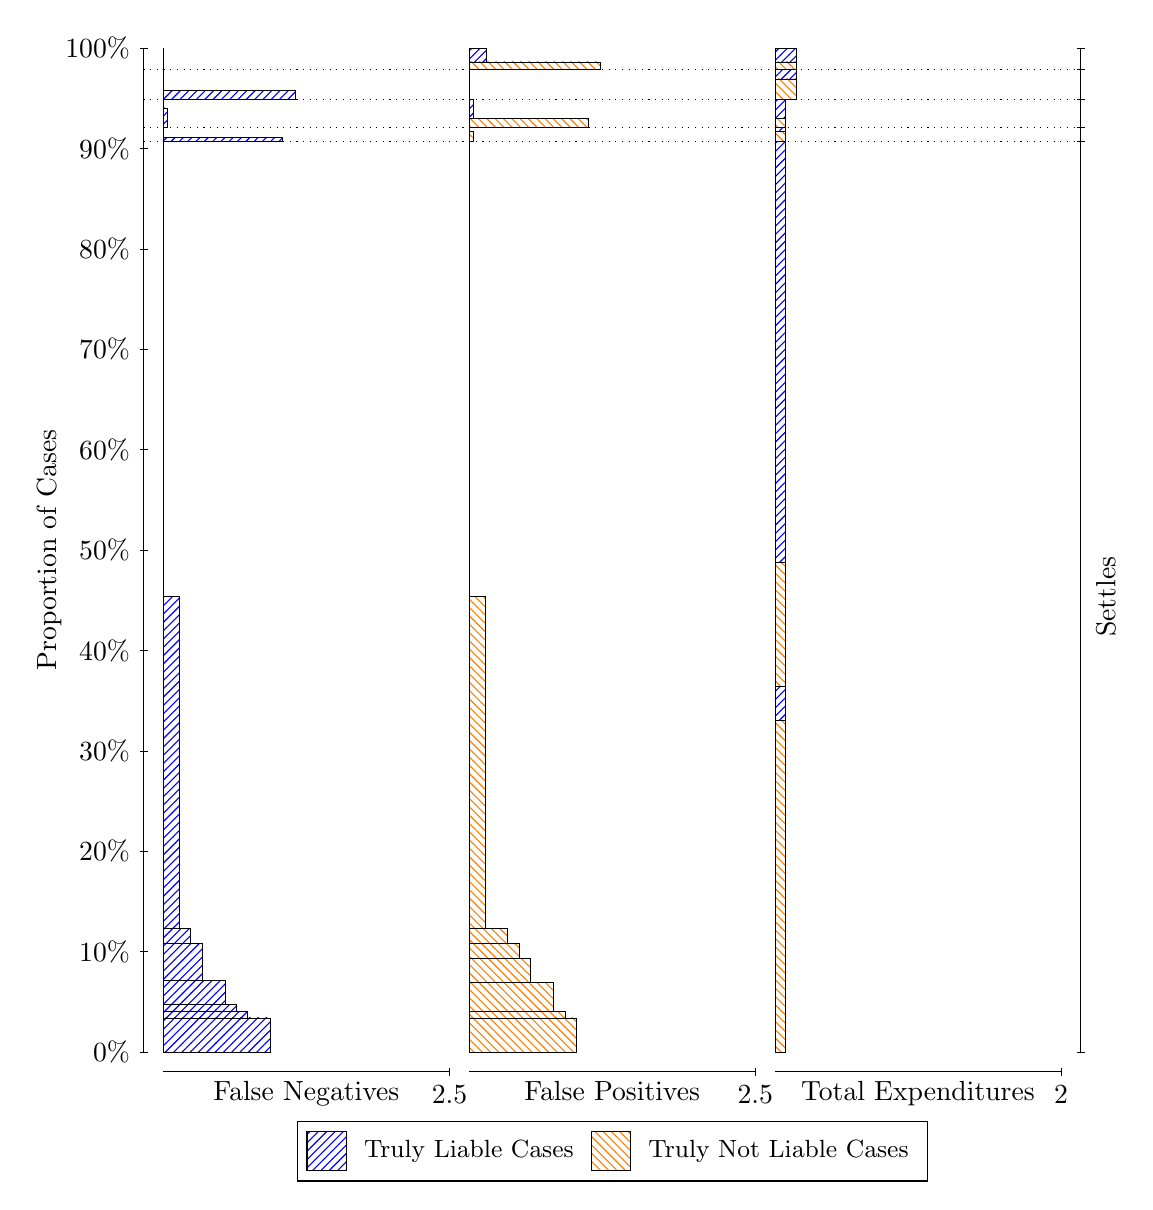
\begin{tikzpicture}
\draw[black, very thin] (1.5,1.75) -- (1.5,14.5);
\node[rotate=90, text=black, anchor=center] at (0.3, 8.125) {Proportion of Cases};
\draw[black, very thin] (1.45,1.75) -- (1.55,1.75);
\node[text=black, anchor=east] at (1.45, 1.75) {0\%};
\draw[black, very thin] (1.45,3.025) -- (1.55,3.025);
\node[text=black, anchor=east] at (1.45, 3.025) {10\%};
\draw[black, very thin] (1.45,4.3) -- (1.55,4.3);
\node[text=black, anchor=east] at (1.45, 4.3) {20\%};
\draw[black, very thin] (1.45,5.575) -- (1.55,5.575);
\node[text=black, anchor=east] at (1.45, 5.575) {30\%};
\draw[black, very thin] (1.45,6.85) -- (1.55,6.85);
\node[text=black, anchor=east] at (1.45, 6.85) {40\%};
\draw[black, very thin] (1.45,8.125) -- (1.55,8.125);
\node[text=black, anchor=east] at (1.45, 8.125) {50\%};
\draw[black, very thin] (1.45,9.4) -- (1.55,9.4);
\node[text=black, anchor=east] at (1.45, 9.4) {60\%};
\draw[black, very thin] (1.45,10.675) -- (1.55,10.675);
\node[text=black, anchor=east] at (1.45, 10.675) {70\%};
\draw[black, very thin] (1.45,11.95) -- (1.55,11.95);
\node[text=black, anchor=east] at (1.45, 11.95) {80\%};
\draw[black, very thin] (1.45,13.225) -- (1.55,13.225);
\node[text=black, anchor=east] at (1.45, 13.225) {90\%};
\draw[black, very thin] (1.45,14.5) -- (1.55,14.5);
\node[text=black, anchor=east] at (1.45, 14.5) {100\%};

\draw[black, very thin] (13.4,1.75) -- (13.4,14.5);
\draw[black, very thin] (13.35,1.75) -- (13.45,1.75);
\node[anchor=west] at (13.35, 1.75) {};
\draw[black, very thin] (13.35,13.315) -- (13.45,13.315);
\node[anchor=west] at (13.35, 13.315) {};
\draw[black, very thin] (13.35,13.493) -- (13.45,13.493);
\node[anchor=west] at (13.35, 13.493) {};
\draw[black, very thin] (13.35,13.849) -- (13.45,13.849);
\node[anchor=west] at (13.35, 13.849) {};
\draw[black, very thin] (13.35,14.224) -- (13.45,14.224);
\node[anchor=west] at (13.35, 14.224) {};
\draw[black, very thin] (13.35,14.5) -- (13.45,14.5);
\node[anchor=west] at (13.35, 14.5) {};

\draw[black, very thin, pattern color=blue, pattern=north east lines] (1.75,1.75) rectangle (3.1125,2.1834);
\draw[black, very thin, pattern color=blue, pattern=north east lines] (1.75,2.1834) rectangle (2.8218,2.2682);
\draw[black, very thin, pattern color=blue, pattern=north east lines] (1.75,2.2682) rectangle (2.6765,2.3531);
\draw[black, very thin, pattern color=blue, pattern=north east lines] (1.75,2.3531) rectangle (2.5312,2.6587);
\draw[black, very thin, pattern color=blue, pattern=north east lines] (1.75,2.6587) rectangle (2.2405,3.1273);
\draw[black, very thin, pattern color=blue, pattern=north east lines] (1.75,3.1273) rectangle (2.0952,3.3198);
\draw[black, very thin, pattern color=blue, pattern=north east lines] (1.75,3.3198) rectangle (1.9498,7.5325);
\draw[black, very thin, pattern color=orange, pattern=north west lines] (1.75,7.5325) rectangle (1.75,13.315);
\draw[black, very thin, pattern color=blue, pattern=north east lines] (1.75,13.315) rectangle (3.2578,13.37);
\draw[black, very thin, pattern color=orange, pattern=north west lines] (1.75,13.37) rectangle (1.75,13.493);
\draw[black, very thin, pattern color=blue, pattern=north east lines] (1.75,13.493) rectangle (1.8045,13.74);
\draw[black, very thin, pattern color=orange, pattern=north west lines] (1.75,13.74) rectangle (1.75,13.849);
\draw[black, very thin, pattern color=blue, pattern=north east lines] (1.75,13.849) rectangle (3.4213,13.964);
\draw[black, very thin, pattern color=orange, pattern=north west lines] (1.75,13.964) rectangle (1.75,14.224);
\draw[black, very thin, pattern color=orange, pattern=north west lines] (1.75,14.224) rectangle (1.75,14.324);
\draw[black, very thin, pattern color=blue, pattern=north east lines] (1.75,14.324) rectangle (1.75,14.5);
\draw[black, very thin, pattern color=orange, pattern=north west lines] (5.6333,1.75) rectangle (6.9958,2.1834);
\draw[black, very thin, pattern color=orange, pattern=north west lines] (5.6333,2.1834) rectangle (6.8505,2.2683);
\draw[black, very thin, pattern color=orange, pattern=north west lines] (5.6333,2.2683) rectangle (6.7052,2.6291);
\draw[black, very thin, pattern color=orange, pattern=north west lines] (5.6333,2.6291) rectangle (6.4145,2.9348);
\draw[black, very thin, pattern color=orange, pattern=north west lines] (5.6333,2.9348) rectangle (6.2692,3.1273);
\draw[black, very thin, pattern color=orange, pattern=north west lines] (5.6333,3.1273) rectangle (6.1238,3.3198);
\draw[black, very thin, pattern color=orange, pattern=north west lines] (5.6333,3.3198) rectangle (5.8332,7.5324);
\draw[black, very thin, pattern color=blue, pattern=north east lines] (5.6333,7.5324) rectangle (5.6333,13.315);
\draw[black, very thin, pattern color=orange, pattern=north west lines] (5.6333,13.315) rectangle (5.6878,13.438);
\draw[black, very thin, pattern color=blue, pattern=north east lines] (5.6333,13.438) rectangle (5.6333,13.493);
\draw[black, very thin, pattern color=orange, pattern=north west lines] (5.6333,13.493) rectangle (7.1412,13.603);
\draw[black, very thin, pattern color=blue, pattern=north east lines] (5.6333,13.603) rectangle (5.6878,13.849);
\draw[black, very thin, pattern color=orange, pattern=north west lines] (5.6333,13.849) rectangle (5.6333,14.109);
\draw[black, very thin, pattern color=blue, pattern=north east lines] (5.6333,14.109) rectangle (5.6333,14.224);
\draw[black, very thin, pattern color=orange, pattern=north west lines] (5.6333,14.224) rectangle (7.3047,14.324);
\draw[black, very thin, pattern color=blue, pattern=north east lines] (5.6333,14.324) rectangle (5.8513,14.5);
\draw[black, very thin, pattern color=orange, pattern=north west lines] (9.5167,1.75) rectangle (9.6529,5.9626);
\draw[black, very thin, pattern color=blue, pattern=north east lines] (9.5167,5.9626) rectangle (9.6529,6.3959);
\draw[black, very thin, pattern color=orange, pattern=north west lines] (9.5167,6.3959) rectangle (9.6529,7.9658);
\draw[black, very thin, pattern color=blue, pattern=north east lines] (9.5167,7.9658) rectangle (9.6529,13.315);
\draw[black, very thin, pattern color=orange, pattern=north west lines] (9.5167,13.315) rectangle (9.6529,13.438);
\draw[black, very thin, pattern color=blue, pattern=north east lines] (9.5167,13.438) rectangle (9.6529,13.493);
\draw[black, very thin, pattern color=orange, pattern=north west lines] (9.5167,13.493) rectangle (9.6529,13.603);
\draw[black, very thin, pattern color=blue, pattern=north east lines] (9.5167,13.603) rectangle (9.6529,13.849);
\draw[black, very thin, pattern color=orange, pattern=north west lines] (9.5167,13.849) rectangle (9.7892,14.109);
\draw[black, very thin, pattern color=blue, pattern=north east lines] (9.5167,14.109) rectangle (9.7892,14.224);
\draw[black, very thin, pattern color=orange, pattern=north west lines] (9.5167,14.224) rectangle (9.7892,14.324);
\draw[black, very thin, pattern color=blue, pattern=north east lines] (9.5167,14.324) rectangle (9.7892,14.5);
\draw[black, dotted] (1.5,13.315) -- (13.4,13.315);
\draw[black, dotted] (1.5,13.493) -- (13.4,13.493);
\draw[black, dotted] (1.5,13.849) -- (13.4,13.849);
\draw[black, dotted] (1.5,14.224) -- (13.4,14.224);
\draw[black, very thin] (1.75,1.5) -- (5.3833,1.5);
\node[text=black, anchor=north] at (3.5667, 1.5) {False Negatives};
\draw[black, very thin] (5.3833,1.45) -- (5.3833,1.55);
\node[text=black, anchor=north] at (5.3833, 1.45) {2.5};

\draw[black, very thin] (5.6333,1.5) -- (9.2667,1.5);
\node[text=black, anchor=north] at (7.45, 1.5) {False Positives};
\draw[black, very thin] (9.2667,1.45) -- (9.2667,1.55);
\node[text=black, anchor=north] at (9.2667, 1.45) {2.5};

\draw[black, very thin] (9.5167,1.5) -- (13.15,1.5);
\node[text=black, anchor=north] at (11.333, 1.5) {Total Expenditures};
\draw[black, very thin] (13.15,1.45) -- (13.15,1.55);
\node[text=black, anchor=north] at (13.15, 1.45) {2};

\node[text=black, centered, rotate=90] at (13.72, 7.5325) {Settles};





\draw (7.449999999999999,1.5) node[draw=none] (baseCoordinate) {};
\begin{scope}[align=center]
        \matrix[scale=0.5, draw=black, below=0.5cm of baseCoordinate, nodes={draw}, column sep=0.1cm]{
            \node[rectangle, draw, minimum width=0.5cm, minimum height=0.5cm, pattern color=blue, pattern=north east lines] {}; &
            \node[draw=none, font=\small, text=black] (B) {Truly Liable Cases}; &
            \node[rectangle, draw, minimum width=0.5cm, minimum height=0.5cm, pattern color=orange, pattern=north west lines] {}; &
            \node[draw=none, font=\small, text=black] (B) {Truly Not Liable Cases}; \\
            };
\end{scope}

\end{tikzpicture}
\end{document}